\documentclass{article}

\usepackage{lmodern}
\usepackage{hyperref}
\usepackage{amsmath}
\usepackage{amssymb}
\usepackage[T1]{fontenc}
\usepackage{color,graphicx}

\begin{document}

\title{Kernel Based Approaches for Change-Point Detection\\ Midway report}
\date{April 3, 2016}
\author{Anirudhan J. Rajagopalan, ajr619}

\maketitle

\newpage

\begin{abstract}
  Electroencephalography (EEG) signals are detected by using electrodes that are applied to the surface of mamals.  A sensitive instrument can show continuous fluctuations of the electric potential between the electrodes.  These potentials are due to the superposition of the electrical activity of tens of thousands of neuron cells lying on the surface areas of the brain~\cite{npsdpm}.  A typical human EEG signal is produced by 36 electrodes placed on the scalp.  This work aims to exploit the spatial relation of the electrodes to identify a Reproducing Kernel Hilbert Space (RKHS) kernel function that will help us find the change points in the EEG signal data.
\end{abstract}


\section{Change point detection}
\subsection{Stationary process}
A stationary process is a stochastic process whose joint probability distribution does not change when shifted in time.  Consequently, parameters that define the process such as mean ($\mu$), standard deviation ($\sigma$) remain constant

\subsection{Change points}
A change point in a time series is the times at which the probability distribution of the time series changes.  A change point detection problem involves detecting whether or not a change has occured, and identifying the times at which such changes occured.

Change points can be identified when the parameters defining the stationary process, such as mean ($\mu$) and standard deviation ($\sigma$) changes.  We discuss ways to identify change points when mean of the process changes.
\subsection{Offline Change point detection}
Offline change point detection or retrospective change point detection methods has the complete data available at the beginning of the program.

\subsubsection{Univariate Time series}
Lets assume a time series of observations $x_{1}, x_{2}, \ldots, x_{n} $ of independent random variables with parameters $(\mu_{1}, \sigma_{1}^{2}), (\mu_{2}, \sigma_{2}^{2}), \ldots, (\mu_{n}, \sigma_{n}^{2}) $.
Also lets assume that each of the observation $ x_{i} $ is normally distributed with mean $ \mu $ and common variance $\sigma^{2} \forall i \in 1, 2, \ldots ,n $.
When there is no change in mean, the hypothesis of stability (null hypothesis) is defined as
\begin{align}
  H_{0} : \mu_{1} = \mu_{2} = \cdots =  \mu_{n} = \mu
\end{align}
Lets suppose that there is a change in the mean in the observations at an unknown point $ K $.  This can be define dy
\begin{align}
  H_{1} : \mu_{1} = \ldots \mu_{k} \ne \mu_{k+1} \ldots =  \mu_{n}
\end{align}
In our experiments we are going to assume that we know $\mu_{1}, \mu_{n} $ and $ \sigma $ are known beforehand (Refer $2.1.1$ of~\cite{birkhauser_pscpa}).

We can find the change poing by using Maximum Likelihood estimates.

Under $H_{0} $,
\begin{align}
  L_{0}(\mu) =& \frac{1}{{(\sqrt{2\pi})}^n} e^{-\sum_{i=1}^{n} \frac{{(x_{i} - \mu)}^2}{2} } \\
\end{align}
and the Maximum likelihood estimator is given by
\begin{align}
  \hat{\mu} =& \bar{x} = \frac{1}{n}\sum_{i=1}^{n} x_{i}
\end{align}

Under $H_{1} $,
\begin{align}
  L_{1}(\mu_{1}, \mu_{n}) =& \frac{1}{{(\sqrt{2\pi})}^n} e^{-(\frac{\sum_{i=1}^{k} {(x_{i} - \mu_{1})}^2 + \sum_{i=k+1}^{n} {(x_{i} - \mu_{n})}^2}{2})} \\
\end{align}
and the Maximum likelihood estimator is given by
\begin{align}
  \hat{\mu_{1}} =& \bar{x_{k}} = \frac{1}{k}\sum_{i=1}^{k} x_{i} \\
  \hat{\mu_{n}} =& \bar{x_{n-k}} = \frac{1}{n-k}\sum_{i=k+1}^{n} x_{i} 
\end{align}

We can use the Maximum likelihood estimator directly to find the change points in the given data.  But calculating the MLE is computationaly intractable.  
An alternate set of equations is given in Chapter 2 of~\cite{birkhauser_pscpa}.  We use the alternate set of equations to find the change points.  The experiments using sample data and its results are shown below.

\subsubsection{Experiments --- Univariate time series}
The offline changepoint detection problem, gives a pretty accurate value for changepoint at k = 300.  The different plots are as displayed below.

\begin{figure}[ht!]
  \centering
  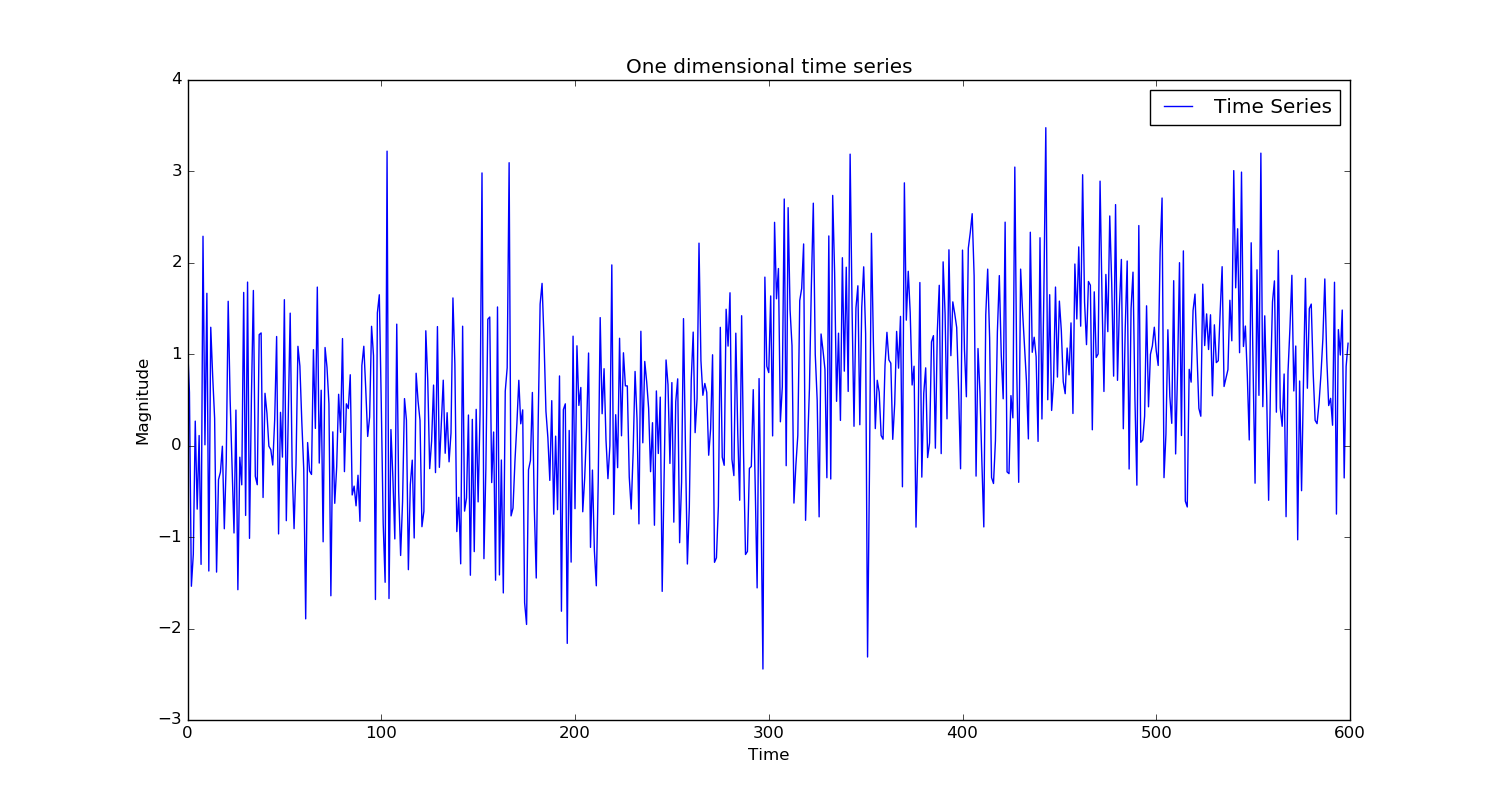
\includegraphics[width=1\textwidth]{images/1d_offline/ts}
  \caption{One dimensional time series.\label{fig:1d_ts}}
\end{figure}

\begin{figure}[ht!]
  \centering
  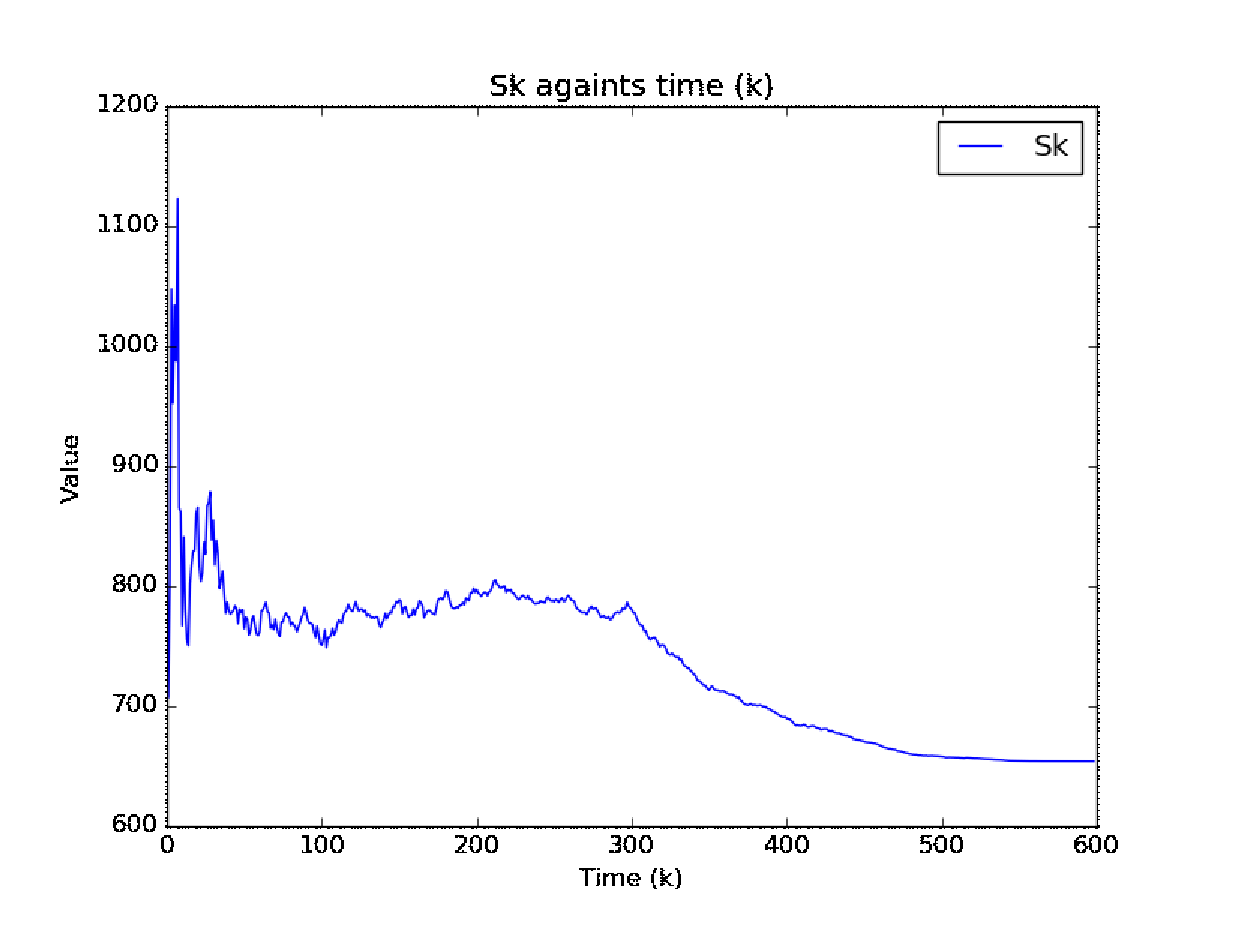
\includegraphics[width=0.75\textwidth]{images/1d_offline/sk}
  \caption{SK values for one dimensional offline detection problem.\label{fig:1d_sk}}
\end{figure}

\begin{figure}[ht!]
  \centering
  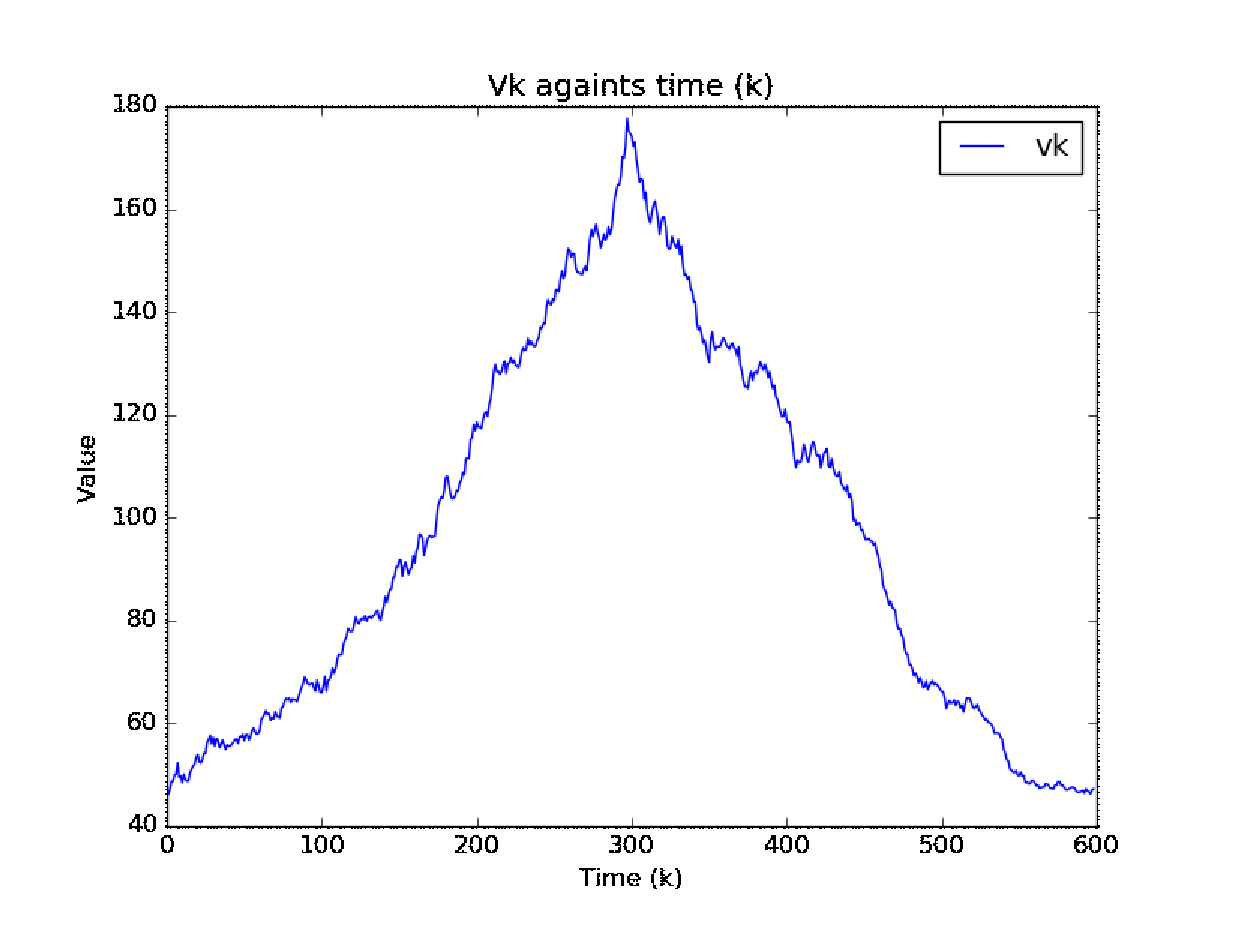
\includegraphics[width=0.75\textwidth]{images/1d_offline/vk}
  \caption{VK values for one dimensional offline detection problem.\label{fig:1d_vk}}
\end{figure}


\subsubsection{Multivariate Time series}

\subsection{Online Change point detection}


\section{Spectral Density}
\subsection{Auto CoVariance Function}
\subsection{Auto Corelation Function}
\subsection{Peridogram}
\subsection{Change points using spectral density}

\bibliographystyle{plain}
\bibliography{references}
\end{document}
